\chapter{Dyskusja rezultatów}

\section{Przykładowe wyniki}
\subsection{Wynik dla przykładu ze wstępu}
Wracając do dziennika zdarzeń przedstawionego w sekcji \ref{sec:event_logs}, a dla którego stworzono przykładowy model i obliczono metryki w sekcji \ref{sec:alignment-calculation}. 
\begin{figure}[!ht]
	\centering{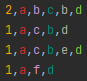
\includegraphics{datasets/v4a6c5l5.png}}
	\caption{\label{fig:flow_chart}Warianty procesu}
\end{figure}

Przy odkrywaniu modelu dla tego wariantu użyto następujących wag poszczególnych metryk: odwzorowanie = 18, złożoność = 2, generalizacja = 2, precyzja = 12, prostota = 2. Model dla tego dziennika zdarzeń znaleziony przy pomocy algorytmu to:
\begin{center}
	\{a\}xor(seq(opt(\{b\})\{c\}\{b\}opt(\{e\}))\{f\})\{d\}
\end{center}
oraz graficznie:

\begin{figure}[!ht]
	\centering{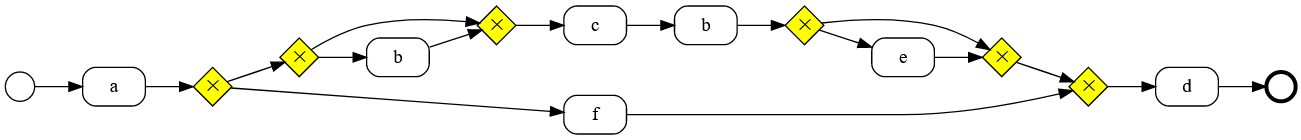
\includegraphics[scale=0.37]{examples/v4a6c5l5.csv_run-686_21_3_21_184242_35664_645567/graphviz.png}}
	\caption{\label{fig:flow_chart}Znaleziony model}
\end{figure}

Do znalezienia modelu potrzebne były 522 generacje, podczas których przeszukano 97771 unikalnych osobników. Zajęło to 1052.8 sekund, używając 4 wątków procesora. Natomiast, metryki mają następujące wartości: 

 \begin{center}
  \begin{tabular}{l}
	Średnia ważona: 0.9550 \\
	Odwzorowanie: 1.0 \\
	Złożoność: 1.0 \\
	Generalizacja: 0.3426 \\
	Precyzja: 0.9875 \\
	Prostota: 0.9231
  \end{tabular}
 \end{center}

Dla porównania poszczególne metryki obliczone w sekcji \ref{sec:alignment-calculation} wynosiły odwzorowanie = 0.9243, złożoność = 0.9706, generalizacja = 0.3997, precyzja = 0.9465, prostota = 0.8333, a średnia ważona używając przyjętych wag, wyniosłaby 0.9001. Używając algorytmu ewolucyjnego, otrzymano więc znacznie lepszy model.

Poniżej zaprezentowano również wykres, na który zaprezentowano zmianę wartości metryk w kolejnych generacjach. Jest on generowany podczas działania algorytmu i kończy się w momencie przerwania działania algorytmu lub po określonej ilości iteracji, a nie znalezienia rozwiązania, gdyż przy algorytmach ewolucyjnych nie można być pewnym, czy znaleziono najlepsze rozwiązanie.
\begin{figure}[!ht]
	\centering{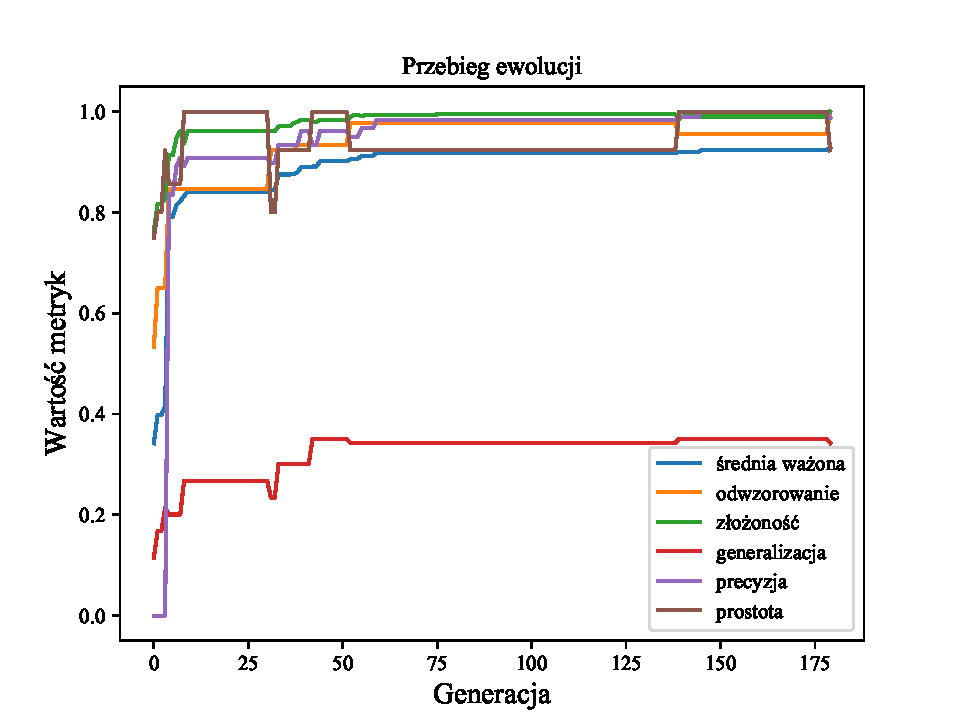
\includegraphics[scale=0.85]{examples/v4a6c5l5.csv_run-648_21_4_23_005638_10340_1/result_graph.pdf}}
	\caption{\label{fig:flow_chart}Przebieg ewolucji}
\end{figure}
\clearpage

\subsection{Inne przykłady działania}

Przykładowe dziennik zdarzeń wzięto z \cite{pm-book}. Część z nich została wygenerowania sztucznie, a część zawiera realne dane. Następnie przerobiono je na warianty procesu. 

\subsubsection{Przykład \#Sztucznie wygenerowany}
Prosty sztucznie wygenerowany przykład. Zawiera 5 unikalnych aktywności, 40 przypadków, 8 wariantów, z których najdłuższy ma 5 zdarzeń. 

\begin{figure}[H]
	\centering{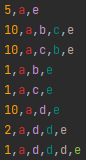
\includegraphics[scale=0.8]{datasets/v8a5c40l5.png}}
	\caption{\label{fig:flow_chart}Warianty procesu}
\end{figure}

Przy odkrywaniu modelu dla tego wariantu użyto następujących wag poszczególnych metryk: odwzorowanie = 8, złożoność = 2, generalizacja = 2, precyzja = 2, prostota = 2. Model dla tego dziennika zdarzeń znaleziony przy pomocy algorytmu to:
\begin{center}
	\{a\}lo2(\{d\})opt(\{b\}\{c\})\{e\}
\end{center}
oraz graficznie:

\begin{figure}[H]
	\centering{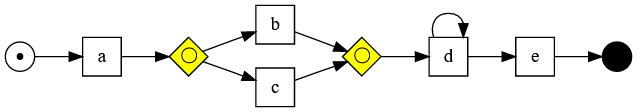
\includegraphics[scale=0.37]{examples/v8a5c40l5.csv_run-24_21_3_6_211037_47336_515221/graphviz.png}}
	\caption{\label{fig:flow_chart}Znaleziony model}
\end{figure}

Do znalezienia modelu potrzebne było 11 generacji, podczas których przeszukano 3636 unikalnych osobników. Zajęło to 75.2 sekund, używając 4 wątków procesora. Natomiast, metryki mają następujące wartości: 

 \begin{center}
  \begin{tabular}{l}
	Średnia ważona: 0.9722 \\
	Odwzorowanie: 1.0 \\
	Złożoność: 1.0 \\
	Generalizacja: 0.7940 \\
	Precyzja: 0.9834 \\
	Prostota: 1.0
  \end{tabular}
 \end{center}
 
\begin{figure}[H]
	\centering{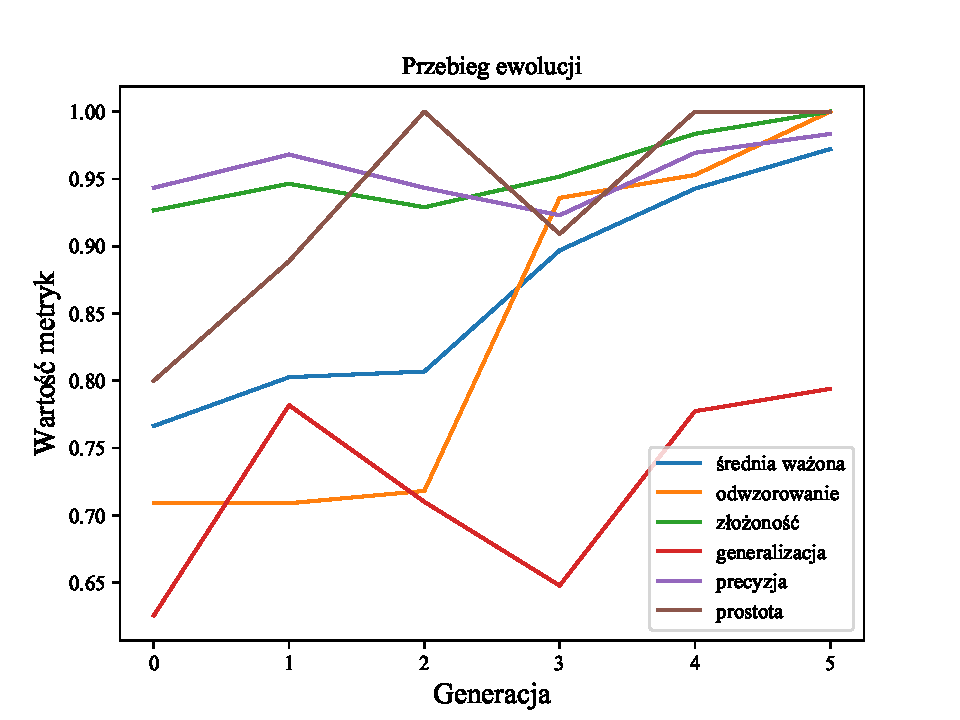
\includegraphics[scale=0.83]{examples/v8a5c40l5.csv_run-24_21_3_6_211037_47336_515221/result_graph.pdf}}
	\caption{\label{fig:flow_chart}Przebieg ewolucji}
\end{figure}

\subsubsection{Przykład \#Obsługa roszczeń w firmie ubezpieczeniowej}
Dziennik danych zawiera dane opisujące obsługa roszczeń w firmie ubezpieczeniowej. Proces może być obsługiwany przez dwie różne działy w Brisbane i Sydney. Możliwe jest połączenie danych dla tych działów, ale nie zrobiono tego, żeby utrudnić odkrywanie modelu.
Przykład składa się z 11 unikalnych aktywności, 3512 przypadków, 12 wariantów, z których najdłuższy ma 9 zdarzeń. 

\begin{figure}[H]
	\centering{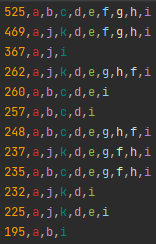
\includegraphics[scale=0.8]{datasets/v12a11c3512l9.png}}
	\caption{\label{fig:flow_chart}Warianty procesu}
\end{figure}

Przy odkrywaniu modelu dla tego wariantu użyto następujących wag poszczególnych metryk: odwzorowanie = 8, złożoność = 2, generalizacja = 2, precyzja = 2, prostota = 2. Model dla tego dziennika zdarzeń znaleziony przy pomocy algorytmu to:
\begin{center}
	\{a\}opt(xor(\{j\}\{b\})\{k\})opt(opt(\{d\}\{e\})\{c\})opt(and(\{f\}\{h\}\{g\}))\{i\}
\end{center}
oraz graficznie:

\begin{figure}[H]
	\centering{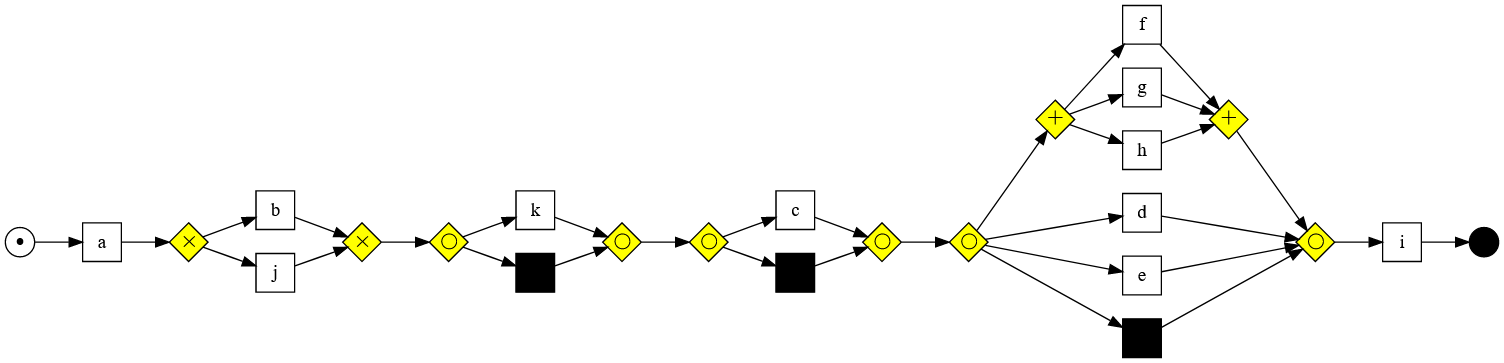
\includegraphics[scale=0.3]{examples/v12a11c3512l9.csv_run-10231_21_3_1_042344_29708_523416/graphviz.png}}
	\caption{\label{fig:flow_chart}Znaleziony model}
\end{figure}

Do znalezienia modelu potrzebne było 4110 generacji. Zajęło to 17157.7 sekund, używając 32 wątków procesora. Natomiast, metryki mają następujące wartości: 

 \begin{center}
  \begin{tabular}{l}
	Średnia ważona: 0.9748 \\
	Odwzorowanie: 1.0 \\
	Złożoność: 1.0 \\
	Generalizacja: 0.9782 \\
	Precyzja: 0.8204 \\
	Prostota: 1.0
  \end{tabular}
 \end{center}
 
\begin{figure}[H]
	\centering{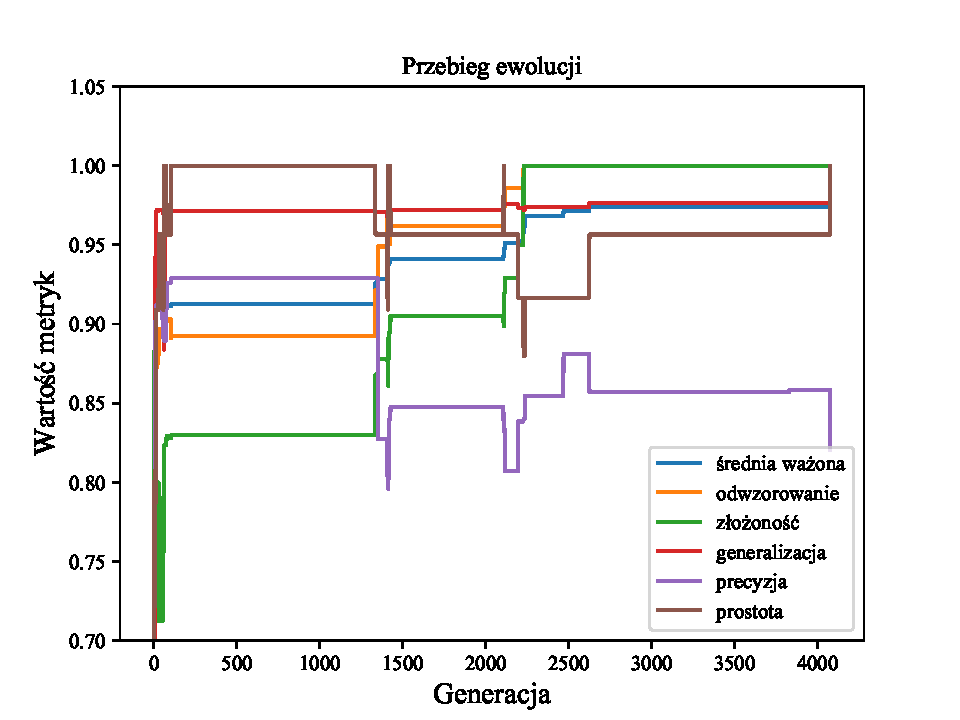
\includegraphics[scale=0.73]{examples/v12a11c3512l9.csv_run-10231_21_3_1_042344_29708_523416/result_graph.pdf}}
	\caption{\label{fig:flow_chart}Przebieg ewolucji}
\end{figure}

\subsubsection{Przykład \#Naprawa telefonu}
Dziennik zdarzeń zawiera dane dotyczące procesu naprawy telefonu.
Przykład składa się z 7 unikalnych aktywności, 1000 przypadków, 45 wariantów, z których najdłuższy ma 14 zdarzeń. 

\begin{figure}[H]
	\centering{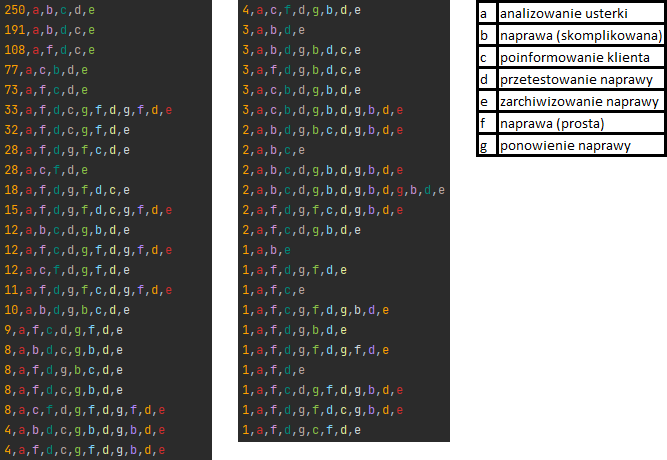
\includegraphics[scale=0.8]{datasets/v45a7c1000l14.png}}
	\caption{\label{fig:flow_chart}Warianty procesu}
\end{figure}

Przy odkrywaniu modelu dla tego wariantu użyto następujących wag poszczególnych metryk: odwzorowanie = 8, złożoność = 2, generalizacja = 2, precyzja = 4, prostota = 1. Model dla tego dziennika zdarzeń znaleziony przy pomocy algorytmu to:
\begin{center}
	\{a\}xor(\{f\}\{b\})and(\{d\}opt(\{c\}))lo3(\{g\}xor(\{f\}\{b\})and(\{d\}opt(\{c\})))\{e\}
\end{center}
oraz graficznie:

\begin{figure}[H]
	\centering{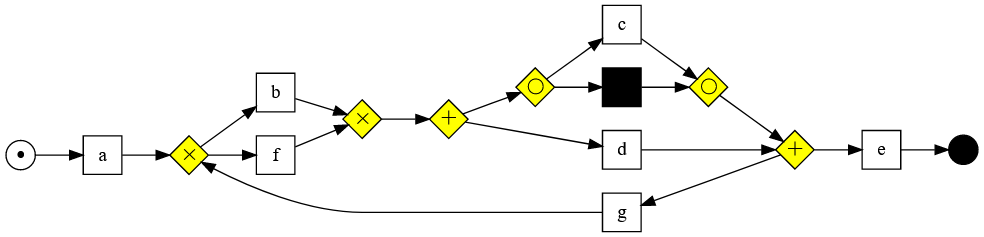
\includegraphics[scale=0.37]{examples/v45a7c1000l14.csv_run-1366_21_3_6_143708_2144_563150/graphviz.png}}
	\caption{\label{fig:flow_chart}Znaleziony model}
\end{figure}

Do znalezienia modelu potrzebne było 436 generacji. Zajęło to 4675.0 sekund, używając 32 wątków procesora. Natomiast, metryki mają następujące wartości: 

 \begin{center}
  \begin{tabular}{l}
	Średnia ważona: 0.9859 \\
	Odwzorowanie: 0.9896 \\
	Złożoność: 0.9891 \\
	Generalizacja: 0.9614 \\
	Precyzja: 0.9859 \\
	Prostota: 1.0
  \end{tabular}
 \end{center}
 
\begin{figure}[H]
	\centering{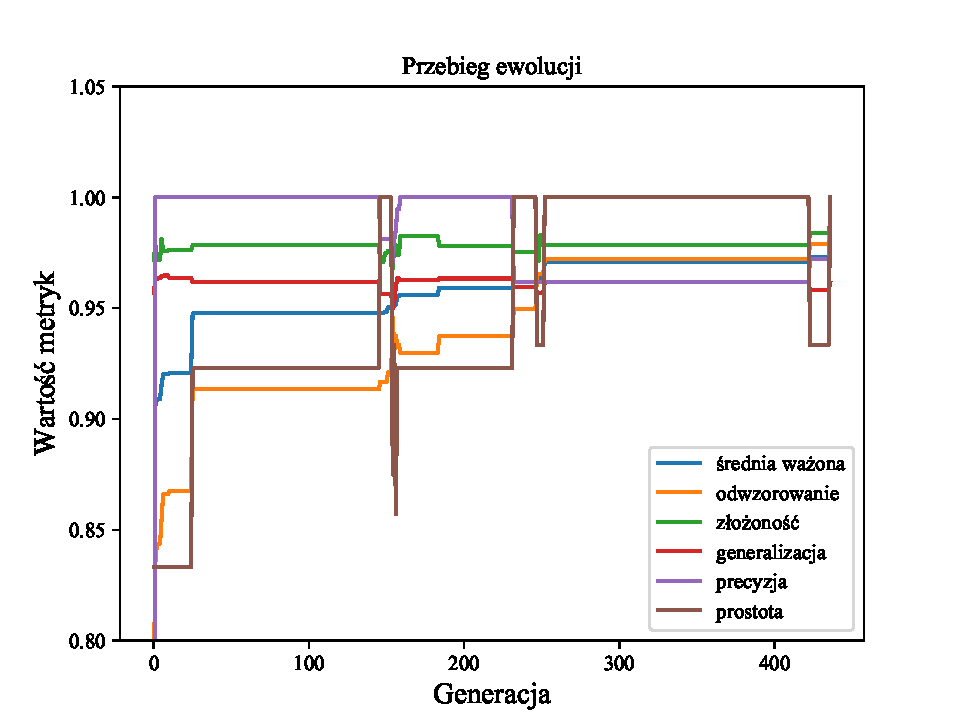
\includegraphics[scale=0.72]{examples/v45a7c1000l14.csv_run-1366_21_3_6_143708_2144_563150/result_graph.pdf}}
	\caption{\label{fig:flow_chart}Przebieg ewolucji}
\end{figure}

\subsubsection{Przykład \#Obsługa wniosku o odszkodowanie}
\label{sec:example5}
Dziennik zdarzeń zawiera dane obsługi wniosku o odszkodowanie.
Przykład składa się z 8 unikalnych aktywności, 1391 przypadków, 21 wariantów, z których najdłuższy ma 17 zdarzeń. 
\begin{figure}[!ht]
	\centering{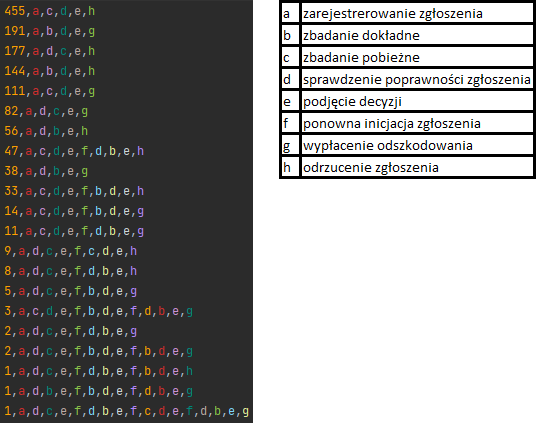
\includegraphics[scale=0.8]{datasets/v21a81391l17.png}}
	\caption{\label{fig:flow_chart}Warianty procesu}
\end{figure}

Przy odkrywaniu modelu dla tego wariantu użyto następujących wag poszczególnych metryk: odwzorowanie = 8, złożoność = 2, generalizacja = 2, precyzja = 2, prostota = 2. Model dla tego dziennika zdarzeń znaleziony przy pomocy algorytmu to:
\begin{center}
	\{a\}lo1(\{f\}and(\{d\}xor(\{b\}\{c\}))\{e\})xor(\{g\}\{h\})
\end{center}
oraz graficznie:

\begin{figure}[H]
	\centering{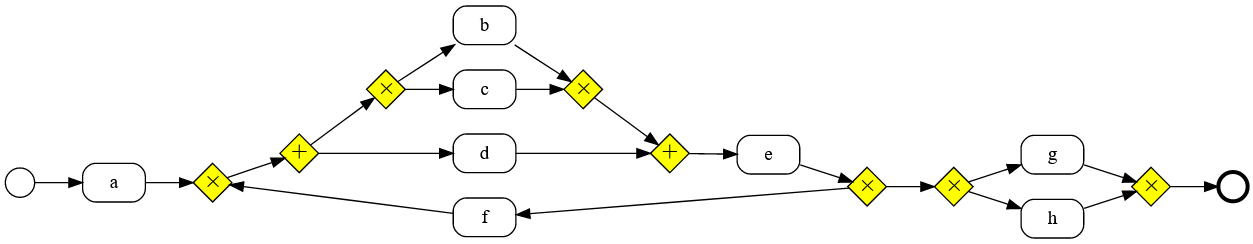
\includegraphics[scale=0.37]{examples/v21a81391l17.csv_run-15614_21_3_1_225455/graphviz.png}}
	\caption{\label{fig:flow_chart}Znaleziony model}
\end{figure}

Do znalezienia modelu potrzebne było 685 generacji. Zajęło to 14728.9 sekund, używając 1 wątku procesora. Natomiast, metryki mają następujące wartości: 

 \begin{center}
  \begin{tabular}{l}
	Średnia ważona: 0.9940 \\
	Odwzorowanie: 1.0 \\
	Złożoność: 1.0 \\
	Generalizacja: 0.9624 \\
	Precyzja: 0.9899 \\
	Prostota: 1.0
  \end{tabular}
 \end{center}
 
\begin{figure}[H]
	\centering{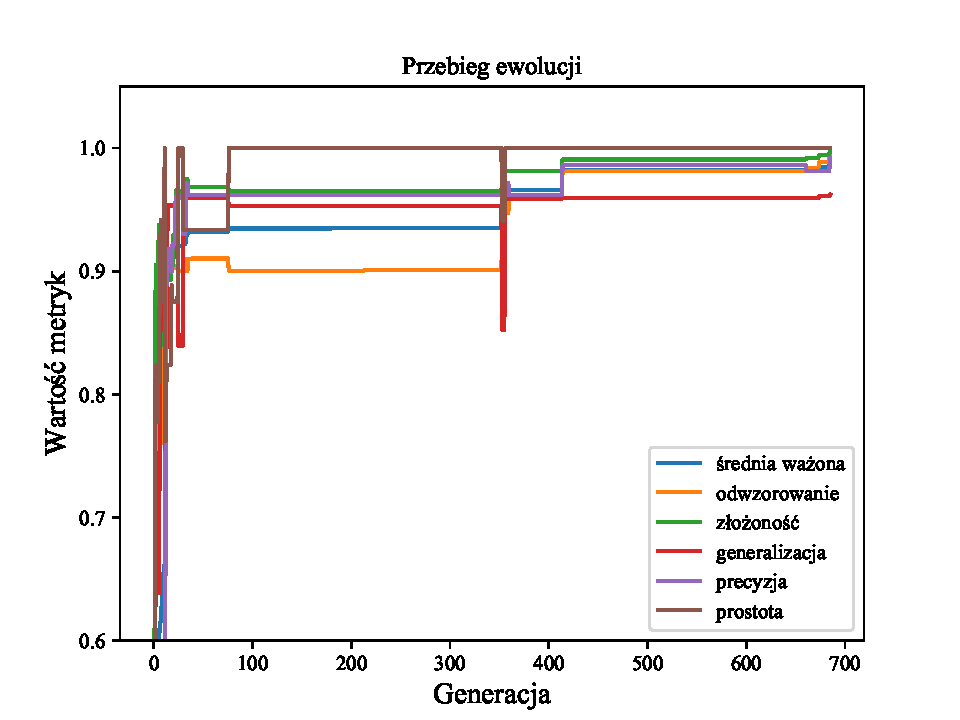
\includegraphics[scale=0.83]{examples/v21a81391l17.csv_21_4_13_201133_15092_996333/result_graph.pdf}}
	\caption{\label{fig:flow_chart}Przebieg ewolucji}
\end{figure}

\section{Wyniki w zależności od przyjętych wag poszczególnych metryk}

\subsection{Brak poszczególnych metryk}
Odwzorowanie jest kluczowe, gdyż jest jedyną metryką, która sprawdza zgodność modelu z dziennikiem zdarzeń i bez tej metryki model byłby pozbawiony wartości. Pozostałe metryki wpływają na jego jakość. Warto więc sprawdzić jak ich brak wpłynąłby na jego odkryty model.

\subsubsection{Poprawny model}
Wpływ braku poszczególnych metryk został sprawdzony dla podzbioru dziennika zdarzeń z sekcji \ref{sec:example5} uproszczonego poprzez pozbawienie go pętli. Dla porównania przedstawiono poprawny model, odkryty używając wszystkich metryk.
Składa się on z 7 unikalnych aktywności, 1254 przypadków, 8 wariantów, które mają po 5 zdarzeń. 
\begin{figure}[!ht]
	\centering{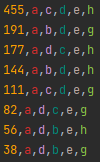
\includegraphics[scale=0.8]{datasets/v8a7c1254l5.png}}
	\caption{\label{fig:flow_chart}Warianty procesu}
\end{figure}

Przy odkrywaniu modelu dla tego wariantu użyto następujących wag poszczególnych metryk: odwzorowanie = 8, złożoność = 2, generalizacja = 2, precyzja = 4, prostota = 2. Model dla tego dziennika zdarzeń znaleziony przy pomocy algorytmu to:
\begin{center}
	\{a\}and(xor(\{c\}\{b\})\{d\})\{e\}xor(\{h\}\{g\})
\end{center}
oraz graficznie:

\begin{figure}[!ht]
	\centering{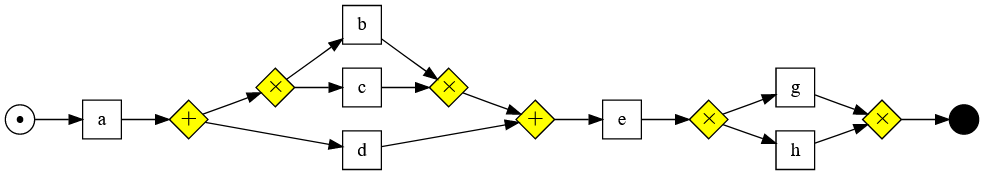
\includegraphics[scale=0.37]{examples/v8a7c1254l5.csv_run-303_21_3_5_003759/graphviz.png}}
	\caption{\label{fig:flow_chart}Znaleziony model}
\end{figure}

Do znalezienia modelu potrzebne były 233 generacje, podczas których przeszukano 41537 unikalnych osobników. Zajęło to 504.2 sekund, używając 4 wątków procesora. Natomiast, metryki mają następujące wartości: 

 \begin{center}
  \begin{tabular}{l}
	Średnia ważona: 0.9960 \\
	Odwzorowanie: 1.0 \\
	Złożoność: 1.0 \\
	Generalizacja: 0.9641 \\
	Precyzja: 1.0 \\
	Prostota: 1.0
  \end{tabular}
 \end{center}

\subsubsection{Brak precyzji}
W kolejnym przykładzie użyto tych samych wag dla poszczególnych metryk, z wyjątkiem precyzji, dla której przyjęto wagę równą 0.
\begin{figure}[!ht]
	\centering{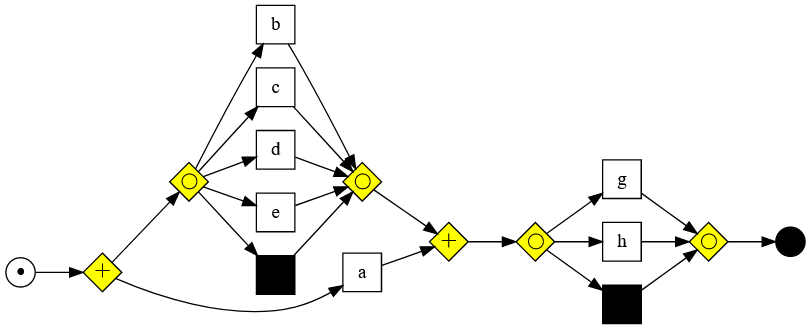
\includegraphics[scale=0.37]{examples/v8a7c1254l5.csv_21_4_13_211038_8672_3/graphviz.png}}
	\caption{\label{fig:v8a7c1254l5.csv_21_4_13_211038_8672_3/graphviz}Znaleziony model}
\end{figure}

Cechą charakterystyczną modelu ze słabą precyzją będzie zastąpienia bramek ,,xor'' bardziej skomplikowanymi bramkami ,,opt'' i ,,and'' oraz niewystarczające ,,dopasowanie się'' do logu, przez co model pozwala na nie mające biznesowego sensu zachowania. Ze względy na mniejszą ilość bramek zazwyczaj potrzebną w modelu ze słabą precyzją oraz z uwagi na większą ilość przypadków uchwyconych w takim modelu i większą szansę na opisanie także tych w logu, wygenerowanie modelu mniej precyzyjnego jest łatwiejsze.
 
Poniżej zaprezentowano średnią ważoną, gdyby przyjąć wagi metryk z poprawnego modelu oraz wartości poszczególnych metryk. 
 \begin{center}
  \begin{tabular}{l}
	Średnia ważona: 0.9289 \\
	Odwzorowanie: 1.0 \\
	Złożoność: 1.0 \\
	Generalizacja: 0.9641 \\
	Precyzja: 0.6982 \\
	Prostota: 1.0
  \end{tabular}
 \end{center}
 
\subsubsection{Brak generalizacji i prostoty}
\label{sec:no-generalization-and-simplicity}
Brak użycia generalizacji miał niezauważalny wpływ na otrzymany model. Ciężko było znaleźć model, który miałby słabą generalizację. Powodem takiej sytuacji może być duża zależność generalizacji od prostoty, gdyż ciężko o niską wartość generalizacji bez obecności dodatkowych elementów w modelu, co obniży wartość jego prostoty. Z tego powodu w tym przykładzie dla wag obu tych metryk przyjęto wartość 0.

Mimo tego wciąż ciężkie okazało się znalezienie modelu ze słabą generalizacją i precyzją. Wynika to z natury ewolucji gramatycznej, gdyż bardziej prawdopodobne jest wygenerowanie prostszego ciągu znaków, dlatego częściej będziemy otrzymywać proste modele z dobrą generalizacją. Szansa na otrzymanie modelu z wysoką wartością funkcji dopasowania spada ze wzrostem ilości elementów. Niemniej, nadal jest możliwe otrzymanie takiego modelu, więc obecność tych metryk nie jest zupełnie bez znaczenia.

Cechą charakterystyczną modelu ze słabą generalizacją będzie zastąpienia bramek ,,and'' i ,,opt'' prostszymi bramkami ,,xor'' oraz nadmierne ,,dopasowanie się'' do jak największej ilości pojedynczych wariantów w logu, przez co nieuchwycone mogą zostać brakujące w logu zachowania.

\begin{figure}[H]
	\centering{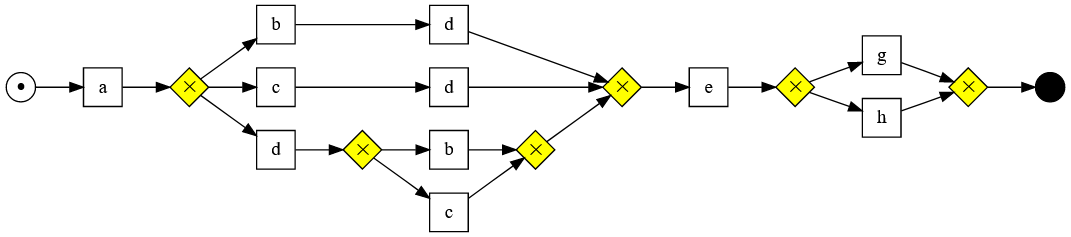
\includegraphics[scale=0.37]{no-generalization-and-simplicity.png}}
	\caption{\label{fig:no-generalization-and-simplicity}Znaleziony model}
\end{figure}

Poniżej zaprezentowano średnią ważoną, gdyby przyjąć wagi metryk z poprawnego modelu oraz wartości poszczególnych metryk. Co ciekawe generalizacja, wciąż nie jest dużo niższa niż w poprawnym modelu.
 
 \begin{center}
  \begin{tabular}{l}
	Średnia ważona: 0.9697 \\
	Odwzorowanie: 1.0 \\
	Złożoność: 1.0 \\
	Generalizacja: 0.9498 \\
	Precyzja: 1.0 \\
	Prostota: 0.7778
  \end{tabular}
 \end{center}

\subsection{Wpływ złożoności na wynik}
W sekcji \ref{sec:additional-metric-complexity} przewidywano dwa aspekty ewolucji, na które powinna wpłynąć złożoność. Były to czas trwania obliczania pojedynczej generacji oraz poprawa ogólnej jakości modelu poprzez unikania lokalny ekstremów na wczesnych etapach ewolucji. 

Celem sprawdzenia tej hipotezy, przetestowano algorytm dla przykładu z sekcji \ref{sec:example5}. Został on  uruchomiony 35 razy ze złożonością równą 0 i 36 ze złożonością równą 2. Wszystkie modele ewoluowano przez 1000 pokoleń, gdyż po takiej ilości generacji jest małe prawdopodobieństwo, że nastąpią kolejne zmiany w modelu. 

Ostatecznie użyto 4 różnych konfiguracji i oprócz złożoności zmieniano też wagę precyzji, z uwagi na to, że jest to najbliższa złożoności metryka i pozwoliło to na zbadanie, jak bardzo zależne od siebie są te dwie metryki. W sekcji \ref{sec:no-generalization-and-simplicity} pokazano, że generalizacja i prostota mają mały wpływ na przebieg ewolucji, dlatego pozostały one stałe podczas tego eksperymentu.

Ostatecznie przy odkrywaniu modelu dla tego wariantu użyto następujących wag poszczególnych metryk: odwzorowanie = 8, generalizacja = 2, prostota = 2 i dwie zmienne precyzja równa 2 lub 4 oraz złożoność równa 0 lub 2. 

Pierwszy aspektem, który zbadano, był czas trwania ewolucji. Na rysunku \ref{fig:total_timemulti4} przedstawiono, jak na czas ewolucji wpływają poszczególne konfiguracje parametrów.  

\begin{figure}[H]
	\centering{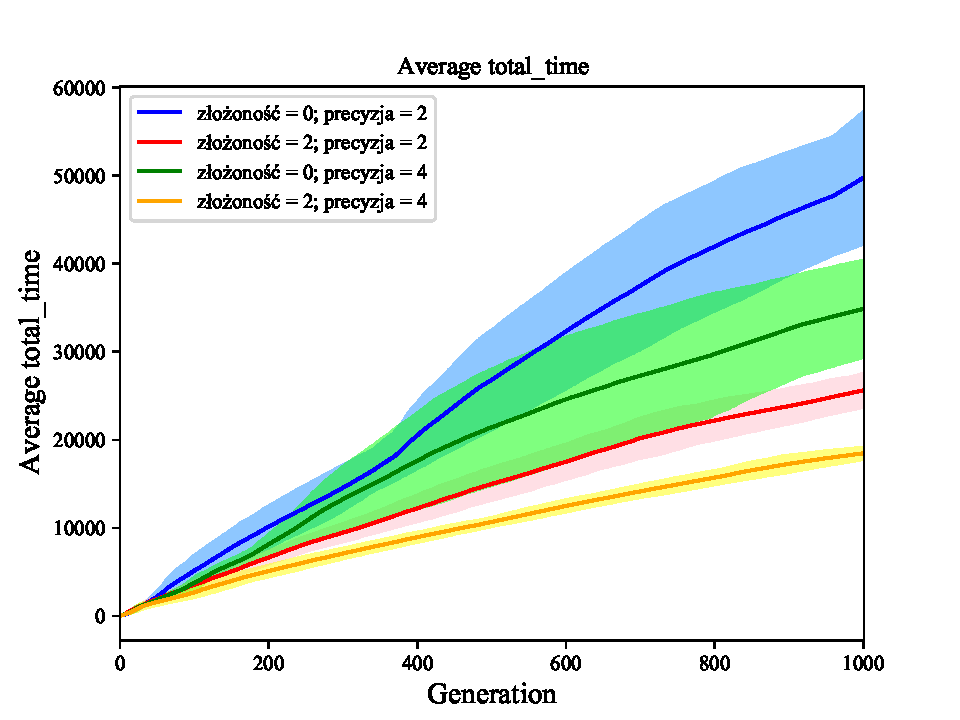
\includegraphics[scale=0.6]{total_timemulti4.pdf}}
	\caption{\label{fig:total_timemulti4}Średni czas i odchylenie standardowe trwania ewolucji}
\end{figure}

 \begin{center}
  \begin{tabular}{ll}
	Czas dla złożoności = 0 i precyzja = 2: & 50600 $\pm$ 6670, \\
	Czas dla złożoności = 0 i precyzja = 4: & 32800	$\pm$ 5960 \\
	Czas dla złożoności = 2 i precyzja = 2: & 24700 $\pm$ 2300 \\
	Czas dla złożoności = 2 i precyzja = 4: & 18300 $\pm$ 657 
  \end{tabular}
 \end{center}
 
Można zauważyć, że zarówno złożoność, jaki i precyzja wpływają na czas ewolucji, a im wyższa waga tych metryk, tym krócej trwa ewolucja. Metryki te mogą być używane razem, a używanie złożoność umożliwia dodatkowe przyspieszenie algorytmu.

Przeanalizowano również, jak zmieniały się wartości poszczególnych metryk i ich średnia ważona. Na rysunku \ref{fig:total_timemulti4} dla poprawy czytelności i lepszego zrozumienia rezultatów pominięto rolę precyzji i skupiono się jedynie na wpływie złożoności.

Warto zaznaczyć, że licząc średnią, nie wzięto pod uwagę złożoności, gdyż jest to parametr, który w założeniu ma służyć jednie usprawnieniu procesu ewolucji, a nie służyć do oceny końcowego modelu. Użyto wagi precyzji równej 4.

\begin{figure}[H]
	\centering{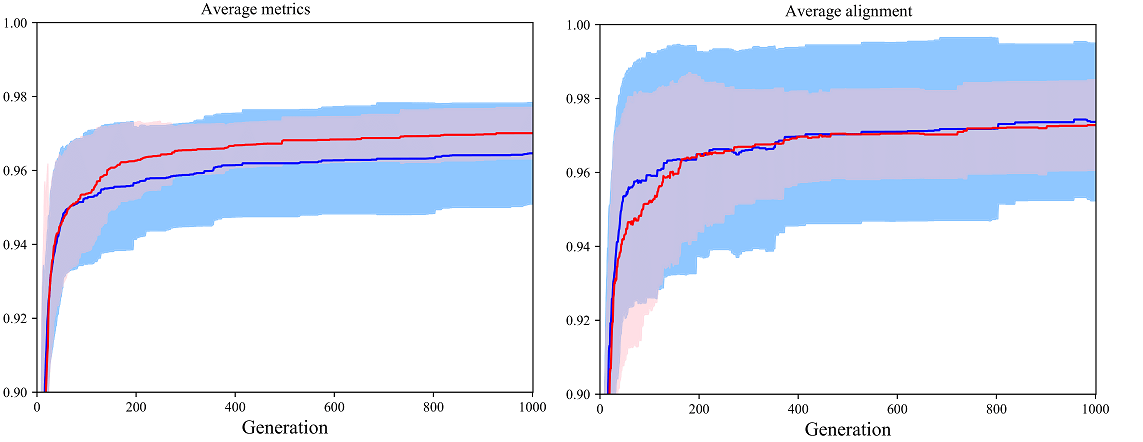
\includegraphics[scale=0.5]{complexity-summary-part1.png}}
\end{figure}

\begin{figure}[H]
	\centering{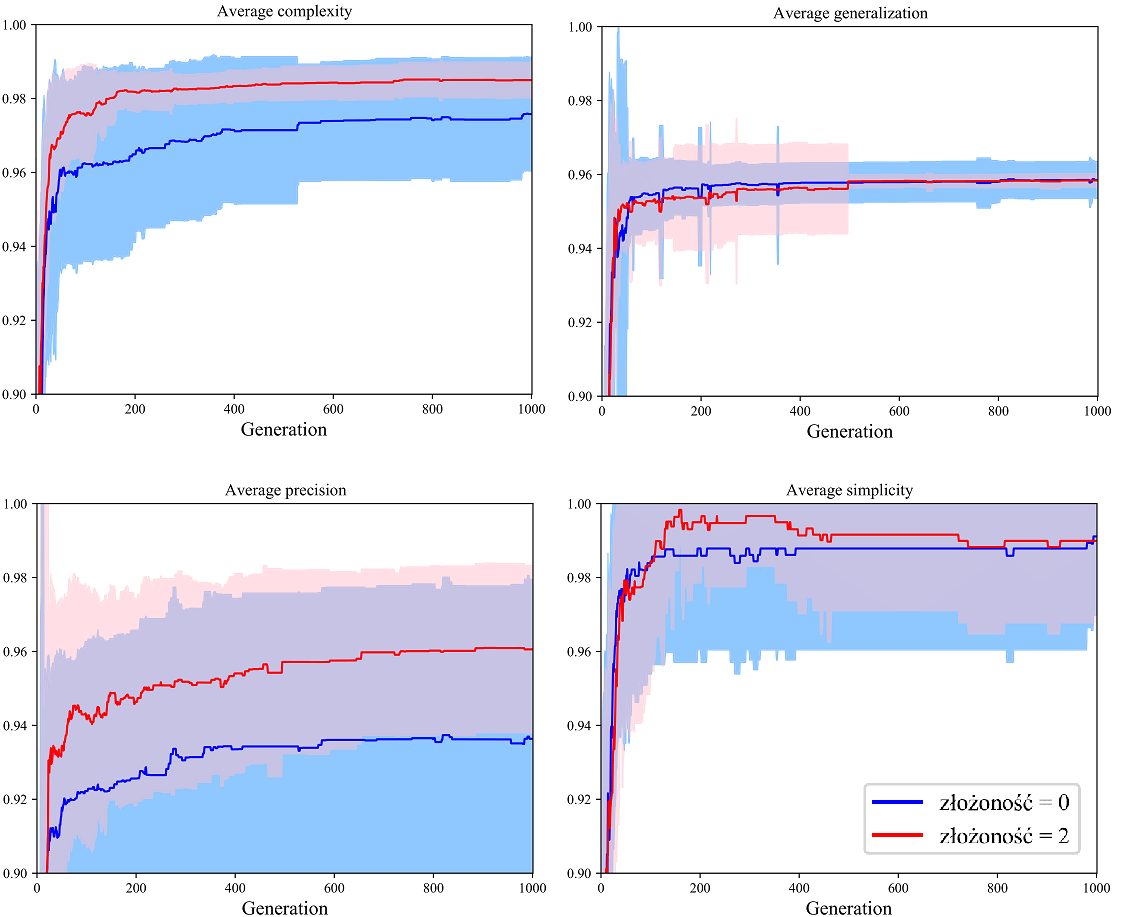
\includegraphics[scale=0.5]{complexity-summary-part23.png}}
	\caption{\label{fig:complexity-summary}Średnie wartości i odchylenie standardowe poszczególnych metryk}
\end{figure}

 \begin{center}
  \begin{tabular}{lll}
  					& Złożoność & Brak złożoności \\
	Średnia ważona: & 0.970 $\pm$ 0.0069 & 0.965 $\pm$ 0.0136 \\ 
	Odwzorowanie: & 0.973 $\pm$ 0.0122 & 0.974 $\pm$ 0.0211 \\
	Złożoność: & 0.985 $\pm$ 0.0048 & 0.976 $\pm$ 0.0152 \\
	Generalizacja: & 0.958 $\pm$ 0.0018 & 0.959 $\pm$ 0.0049 \\
	Precyzja: & 0.961 $\pm$ 0.0224 & 0.935 $\pm$ 0.0432 \\
	Prostota: & 0.989 $\pm$ 0.0233 & 0.991 $\pm$ 0.0212
  \end{tabular}
 \end{center}

Nie udało się stwierdzić zdecydowanego wpływu złożoności na jakość modelu, jednak można zauważyć kilka interesujących różnic, które zgadzają się z intuicją. Otrzymany model jest średnio lepszy, kiedy używa się złożoności, a wpływ na to ma głównie fakt, że jest on bardziej precyzyjny. Warto też, zauważyć, że w takim przypadku we wczesnych generacjach model jest prostszy, ale ma gorsze odwzorowanie, a dopiero z czasem staje się bardziej skomplikowany. Niestety, złożoność zdaje się nie mieć wpływu na najważniejszą z metryk, czyli odwzorowanie, jaki i na generalizację. 

W obu przypadkach udało się znaleźć model tożsamy z modelem w przykładzie z sekcji \ref{sec:example5}, który wydaje się optymalny. Najsłabsze modele otrzymywano, używając konfiguracji bez złożoności.

\section{Wnioski dotyczące ewolucji}
Analizując czasy ewolucji dla przedstawionych przykładów, można zauważyć, że na wzrost czasu oraz ilości generacji potrzebny do znalezienia rozwiązania, wpływa bardziej ilość unikalnych aktywności oraz długość zdarzeń w pojedynczym wariancie niż ich ilość. Algorytmy ewolucyjne źle radzą sobie z dużą ilością zmiennych. Można częściowo jednak rozwiązać ten problem poprzez zrównoleglenie obliczeń, na którą w łatwy sposób pozwalają. 

Dobór wag metryk oddziałuje nie tylko na końcowy model, ale także na każdy model - osobnika w populacji na każdym etapie ewolucji, dlatego wagi metryk powinny być dobierane nie tylko pod kątem końcowego rozwiązania, ale także z myślą o tym, czy wybrany zbiór wag pozwoli na otrzymanie tego rezultatu. Na wykresach pokazujących przebieg ewolucji można zaobserwować wiele przykładów gdzie, aby model mógł stać się ogólnie lepszy, konieczne było tymczasowe pogorszenie się, którejś z metryk. Z tego powodu ważne jest, żeby zachować balans pomiędzy nimi i nawet jeśli w pożądane jest zoptymalizowanie końcowego modelu pod kątem konkretnej metryki, należy ustalić ją tak, żeby nie zdominowała całego procesu ewolucji. 

Po eksperymentach można dojść do wniosku, że wybierając metryki, należy się kierować się ich wpływem na proces ewolucji, a nie końcowy rezultat. Powszechnie używane w eksploracji procesów metryki jak generalizacja nie mają dużego wpływu na działanie algorytmu ewolucyjnego, podczas gdy nowe, nieznane metryki jak złożoność niemające zastosowania do oceny końcowego modelu mogą mieć korzystny wpływ na przebieg ewolucji poprzez ukierunkowanie doboru pośrednich osobników we właściwą stronę, co pozwoli znaleźć lepszy finalny model.
